\documentclass[aspectratio=169,10pt]{beamer}

% Modelo básico de diapositivas para a introdución ao Deep Learning.
% Compilar con pdfLaTeX en Overleaf ou nunha instalación TeX Live.

\usetheme{Madrid}
\usecolortheme{default}
\setbeamertemplate{navigation symbols}{}
\setbeamertemplate{caption}[numbered]

\usepackage[T1]{fontenc}
\usepackage[utf8]{inputenc}
\usepackage{lmodern}
\usepackage{amsmath,amssymb}
\usepackage{booktabs}
\usepackage{graphicx}
\usepackage{hyperref}
\usepackage{xurl}
\usepackage{tikz}
\usetikzlibrary{arrows.meta,positioning,shapes.geometric}
\hypersetup{colorlinks=true,urlcolor=blue!60!black,linkcolor=blue!60!black}

\title[Introdución ao Deep Learning]{Deep Learning para a análise de imaxes preclínicas}
\subtitle{Introdución: da intelixencia artificial á aprendizaxe neuronal}
\author{Lois Nodar Corral}
\institute{[Institución / grupo de investigación]}
\date{[Data]}

\begin{document}

% 1
\begin{frame}
  \titlepage
\end{frame}

% 2
\begin{frame}{Obxectivos desta introdución}
  Ao rematar esta parte, deberiamos poder:
  \begin{itemize}
    \item Situar a aprendizaxe automática e as redes neuronais dentro da IA.
    \item Explicar a idea básica dunha neurona artificial e dunha rede neuronal.
    \item Comprender intuitivamente que é unha convolución.
    \item Adestrar unha pequena rede de regresión en PyTorch.
    \item Explicar, a grandes trazos, como aprende a rede.
  \end{itemize}
\end{frame}

% 3
\begin{frame}{Onde encaixa o Deep Learning?}
  \begin{center}
  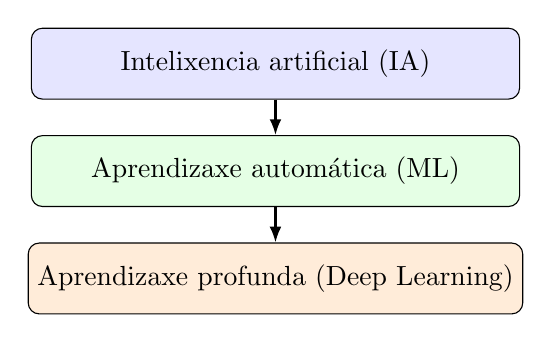
\begin{tikzpicture}[
    box/.style={draw,rounded corners,align=center,minimum width=6.2cm,minimum height=0.9cm},
    arrow/.style={-{Latex[length=2mm]},thick}
  ]
    \node[box,fill=blue!10] (ai) {Intelixencia artificial (IA)};
    \node[box,fill=green!10,below=0.45cm of ai] (ml) {Aprendizaxe automática (ML)};
    \node[box,fill=orange!15,below=0.45cm of ml] (dl) {Aprendizaxe profunda (Deep Learning)};
    \draw[arrow] (ai)--(ml);
    \draw[arrow] (ml)--(dl);
  \end{tikzpicture}
  \end{center}
  \begin{itemize}
    \item \textbf{IA:} métodos para realizar tarefas asociadas á intelixencia.
    \item \textbf{ML:} modelos que aprenden patróns a partir de datos.
    \item \textbf{DL:} modelos baseados en redes neuronais con múltiples capas.
  \end{itemize}
\end{frame}

% 4
\begin{frame}{Exemplos de IA en imaxe médica}
  \begin{itemize}
    \item \textbf{Clasificación:} decidir se unha imaxe contén unha lesión.
    \item \textbf{Detección:} localizar estruturas ou lesións mediante caixas delimitadoras.
    \item \textbf{Segmentación:} asignar unha clase a cada píxel ou vóxel.
    \item \textbf{Reconstrución:} reducir ruído ou reconstruír información ausente.
  \end{itemize}
  \vspace{0.5em}
  \begin{block}{Exemplo do obradoiro}
    A partir dunha TC abdominal, predicir que vóxeles pertencen ao fígado ou a outras estruturas anatómicas.
  \end{block}
\end{frame}

% 5
\begin{frame}{A neurona artificial}
  Unha neurona combina as entradas mediante pesos, engade un termo independente e aplica unha función de activación:
  \[
    z = \sum_{i=1}^{n} w_i x_i + b,
    \qquad a=f(z)
  \]
  \begin{itemize}
    \item \(x_i\): entradas.
    \item \(w_i\): pesos que se aprenden.
    \item \(b\): termo independente (*bias*).
    \item \(f\): función de activación.
  \end{itemize}
  \begin{block}{Idea clave}
    A neurona transforma números de entrada nunha saída; durante o adestramento axústanse os parámetros \(w_i\) e \(b\).
  \end{block}
\end{frame}

\begin{frame}{Esquema dunha neurona}
    \begin{figure}
        \centering
        \includegraphics[width=0.7\linewidth]{neurona.png}
        \caption{v7labs.com}
    \end{figure}
\end{frame}

% 7
\begin{frame}{Que achega unha función de activación?}

\textbf{Non-Linearidade}
  \begin{itemize}
    \item \textbf{ReLU:} \(f(x)=\max(0,x)\). Sinxela e moi usada en redes profundas.
    \item \textbf{Sigmoide:} comprime os valores ao intervalo \((0,1)\).
    \item \textbf{tanh:} comprime os valores ao intervalo \((-1,1)\).
  \end{itemize}
  \begin{block}{Por que importa?}
    Sen non linearidades, apilar capas lineais segue producindo unha transformación lineal: a rede non gañaría capacidade para representar funcións non lineais.
  \end{block}
\end{frame}
% 6
\begin{frame}{Do perceptrón á rede neuronal}
  % \begin{center}
  % \begin{tikzpicture}[
  %   neuron/.style={circle,draw,minimum size=0.58cm},
  %   arrow/.style={-{Latex[length=1.5mm]},thin},
  %   node distance=1.15cm
  % ]
  %   \foreach \i in {1,2,3}
  %     \node[neuron] (i\i) at (0,-\i*0.8) {};
  %   \foreach \i in {1,2,3}
  %     \node[neuron,fill=blue!10] (h\i) at (2.5,-\i*0.8) {};
  %   \foreach \i in {1,2}
  %     \node[neuron,fill=orange!15] (o\i) at (5,-\i*1.2-0.4) {};
  %   \foreach \a in {1,2,3}
  %     \foreach \b in {1,2,3}
  %       \draw[arrow] (i\a)--(h\b);
  %   \foreach \a in {1,2,3}
  %     \foreach \b in {1,2}
  %       \draw[arrow] (h\a)--(o\b);
  %   \node[above=0.1cm of i1] {\scriptsize Entrada};
  %   \node[above=0.1cm of h1] {\scriptsize Capa oculta};
  %   \node[above=0.1cm of o1] {\scriptsize Saída};
  % \end{tikzpicture}
  % \end{center}
  \begin{figure}
      \centering
      \includegraphics[width=0.3\linewidth]{mlp.png}

  \end{figure}
  \begin{itemize}
    \item Un perceptrón é un modelo clásico de clasificación lineal.
    \item Unha rede combina moitas unidades en capas.
    \item As activacións non lineais permiten aprender relacións complexas.
  \end{itemize}
\end{frame}

% 8
\begin{frame}{Que é unha convolución?}
  \begin{itemize}
    \item Un filtro pequeno percorre a imaxe e combina os valores dunha veciñanza.
    \item Cada filtro aprende a responder a determinados patróns locais.
    \item O resultado é un mapa de características (*feature map*).
    \item Os filtros comparten os mesmos pesos en distintas posicións da imaxe.
  \end{itemize}
  \begin{block}{Por que se emprega en imaxe?}
    Permite detectar patróns locais sen ter que aprender un peso distinto para cada píxel de cada posición.
  \end{block}
\end{frame}
\begin{frame}
\begin{figure}
    \centering
    \includegraphics[width=0.5\linewidth]{convolution.png}
    \caption{Esquema funha convolución. analyticsindiamag.com}
\end{figure}
\end{frame}

% 9
\begin{frame}{Práctica: unha rede que aprende unha función}
  \textbf{Tarefa:} aprender a relación aproximada \(y=\sin(x)\) a partir de exemplos con ruído.
  \begin{enumerate}
    \item Xerar os datos de entrada e os valores obxectivo.
    \item Definir unha rede neuronal pequena.
    \item Calcular as predicións e a perda.
    \item Actualizar os parámetros durante varias épocas.
    \item Representar os datos e a curva aprendida.
  \end{enumerate}
  \begin{block}{Pregunta para o grupo}
    Que debería ocorrer coa perda ao longo do adestramento? A perda pode chegar a cero?
  \end{block}
\end{frame}

% 10
\begin{frame}[fragile]{A rede en PyTorch}
\begin{verbatim}
model = nn.Sequential(
    nn.Linear(1, 32),
    nn.ReLU(),
    nn.Linear(32, 1)
)

loss_fn = nn.MSELoss()
optimizer = torch.optim.Adam(
    model.parameters(), lr=0.01
)
\end{verbatim}
  \begin{itemize}
    \item Entrada: un valor \(x\).
    \item Saída: a predición \(\hat y\).
    \item A perda mide a discrepancia entre \(\hat y\) e \(y\).
  \end{itemize}
  \textit{O código completo e a gráfica poden ir nun notebook separado.}
\end{frame}

% 11
\begin{frame}{O ciclo de adestramento}
  \begin{center}
  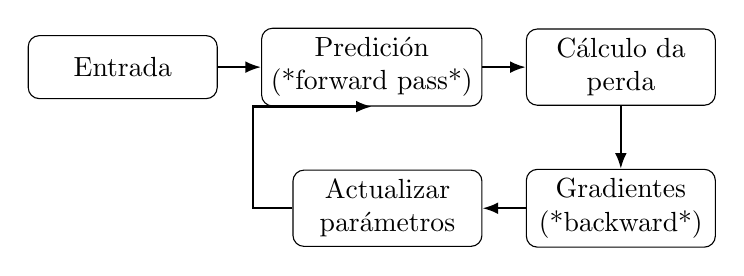
\begin{tikzpicture}[
    block/.style={draw,rounded corners,align=center,minimum width=2.4cm,minimum height=0.8cm},
    arrow/.style={-{Latex[length=2mm]},thick},
    node distance=0.55cm
  ]
    \node[block] (x) {Entrada};
    \node[block,right=of x] (fwd) {Predición\\(*forward pass*)};
    \node[block,right=of fwd] (loss) {Cálculo da\\perda};
    \node[block,below=0.8cm of loss] (back) {Gradientes\\(*backward*)};
    \node[block,left=of back] (update) {Actualizar\\parámetros};
    \draw[arrow] (x)--(fwd);
    \draw[arrow] (fwd)--(loss);
    \draw[arrow] (loss)--(back);
    \draw[arrow] (back)--(update);
    \draw[arrow] (update.west) -- ++(-0.5,0) |- (fwd.south);
  \end{tikzpicture}
  \end{center}
  \begin{enumerate}
    \item A rede produce unha predición.
    \item A función de perda mide o erro.
    \item A retropropagación calcula os gradientes.
    \item O optimizador actualiza os pesos.
  \end{enumerate}
\end{frame}

% 12
\begin{frame}{A función de perda: canto nos equivocamos?}
  Para regresión, unha opción habitual é o erro cuadrático medio (MSE):
  \[
    L=\frac{1}{N}\sum_{i=1}^{N}(\hat y_i-y_i)^2
  \]
  \begin{itemize}
    \item \(y_i\): valor real.
    \item \(\hat y_i\): predición.
    \item Os erros grandes penalízanse máis porque se elevan ao cadrado.
  \end{itemize}
  \begin{block}{Importante}
    Minimizar a perda de adestramento non garante que o modelo funcione ben con datos novos.
  \end{block}
\end{frame}

% 13
\begin{frame}{Regra da cadea e retropropagación}
  A perda depende dos parámetros a través de varias operacións encadeadas. A regra da cadea permite calcular esa dependencia:
  \[
    \frac{\partial L}{\partial w}
    =
    \frac{\partial L}{\partial a}
    \frac{\partial a}{\partial z}
    \frac{\partial z}{\partial w}
  \]
  \begin{itemize}
    \item Cada derivada mide o efecto local dunha variable sobre a seguinte.
    \item O produto enlaza eses efectos ata obter o gradiente respecto dun peso.
    \item A retropropagación aplica esta idea eficientemente a todos os parámetros.
  \end{itemize}
\end{frame}

% 14
\begin{frame}{Como cambian os parámetros?}
  Un paso básico de descenso do gradiente é:
  \[
    w_{\text{novo}}=w_{\text{anterior}}-\eta\frac{\partial L}{\partial w}
  \]
  \begin{itemize}
    \item O gradiente indica a dirección de maior incremento local da perda.
    \item O signo menos indica que avanzamos na dirección contraria.
    \item \(\eta\) é a taxa de aprendizaxe (*learning rate*).
  \end{itemize}
  Se a taxa é demasiado grande, o adestramento pode volverse inestable; se é demasiado pequena, pode avanzar moi amodo.
\end{frame}

% 15
\begin{frame}{Subaxuste e sobreaxuste}
  \begin{columns}[T]
    \column{0.48\textwidth}
      \textbf{Subaxuste (*underfitting*)}
      \begin{itemize}
        \item Modelo demasiado simple ou pouco adestrado.
        \item Erro alto en adestramento e validación.
      \end{itemize}
    \column{0.48\textwidth}
      \textbf{Sobreaxuste (*overfitting*)}
      \begin{itemize}
        \item O modelo aprende tamén o ruído dos datos.
        \item Erro baixo en adestramento, pero alto en validación.
      \end{itemize}
  \end{columns}
  \begin{block}{Obxectivo}
    Aprender patróns que xeneralicen a datos que o modelo non viu durante o adestramento.
  \end{block}
\end{frame}

% 16
\begin{frame}{Por que separar os datos?}
  \begin{itemize}
    \item \textbf{Adestramento:} axusta os parámetros do modelo.
    \item \textbf{Validación:} axuda a escoller configuracións e detectar sobreaxuste.
    \item \textbf{Proba (*test*):} estima o rendemento final con datos non usados para axustar o modelo.
  \end{itemize}
  \begin{alertblock}{En imaxe médica}
    As imaxes dunha mesma persoa ou animal non deberían repartirse inadvertidamente entre adestramento e proba: iso pode producir fuga de información e estimacións demasiado optimistas.
  \end{alertblock}
\end{frame}

% 17
\begin{frame}{Da regresión á segmentación médica}
  \begin{itemize}
    \item A regresión predí un valor numérico.
    \item A clasificación predí unha clase para cada exemplo.
    \item A segmentación predí unha clase para cada píxel ou vóxel.
  \end{itemize}
  \begin{center}
    \fbox{\parbox{0.8\textwidth}{\centering
    \todo{Engadir unha TC abdominal, unha máscara de referencia e a predición da rede}
    }}
  \end{center}
  A lóxica básica de aprendizaxe é semellante; cambian a arquitectura, a función de perda, os datos e as métricas.
\end{frame}

% 18
\begin{frame}{Recursos para seguir aprendendo}
  \small
  \begin{itemize}
    \item Dive into Deep Learning: \url{https://d2l.ai/}
    \item Neural Networks: Zero to Hero (Andrej Karpathy): \url{https://github.com/karpathy/nn-zero-to-hero}
    \item PyTorch: \url{https://pytorch.org/tutorials/}
    \item U-Net (artigo orixinal): \url{https://arxiv.org/abs/1505.04597}
    \item MONAI: \url{https://monai.io/}
    \item Tutorial Swin UNETR para BTCV: \url{https://github.com/Project-MONAI/tutorials/blob/main/3d_segmentation/swin_unetr_btcv_segmentation_3d.ipynb}
  \end{itemize}
\end{frame}

% 19
\begin{frame}{Resumo}
  \begin{itemize}
    \item O Deep Learning é unha parte da aprendizaxe automática.
    \item As redes neuronais aprenden axustando parámetros a partir de exemplos.
    \item A perda mide o erro; os gradientes indican como cambiala.
    \item A retropropagación calcula os gradientes e o optimizador actualiza os parámetros.
    \item Para confiar nos resultados, cómpre avaliar a xeneralización e coñecer as limitacións dos datos.
  \end{itemize}
  \vfill
  \centering
  \Large Preguntas?
\end{frame}

\end{document}
"""

path = Path("/mnt/data/introducion_deep_learning_galego.tex")
path.write_text(content, encoding="utf-8")
print(f"Ficheiro creado: {path}")